\documentclass[12pt,a4paper]{report}
%\usepackage{ucs}
\usepackage[utf8]{inputenc}
\usepackage[T1]{fontenc}
\usepackage{textcomp}
\usepackage[english]{babel}
\usepackage{amsmath}
\usepackage{graphicx}
\usepackage{chngcntr}
\counterwithout{figure}{chapter}
\counterwithout{table}{chapter}

% \usepackage[backend=biber,%
%             style=ieee]{biblatex}
% \addbibresource{quellen.bib}

\title{Specifications - Android Practice App}
\author{Sebastian Bellitto}

\graphicspath{ {./diagrams/} }

\renewcommand{\arraystretch}{1.5}
\renewcommand{\tabcolsep}{0.2cm}

\makeatletter
\usepackage[pdfauthor={\@author},%
            pdftitle={\@title},%
            pdftex]{hyperref}
\makeatother

\begin{document}

\maketitle

\setlength{\parindent}{0pt}
\setlength{\parskip}{1.2ex plus 0.5ex minus 0.2ex}

\tableofcontents
\newpage

\chapter{Overview}\label{c1}
\section{Purpose and Goal of the Application}\label{c1-1}
The App should help with organizing and following a structured musical practice routine.
It should allow for planning practicing sessions and guiding the user through practices.

In future development a web-app version could be added and also extend the app to iOS.
The web-app focus would be on building custom practices and letting teachers manage students practices.

\section{Users and Target Groups}\label{c1-2}
For the first iteration of the app the target groups would be musicians, be it students, professionals or teachers.

In the case that the extended web-app feature mentioned in \ref{c1-1} be implemented, a second main target group would be the teachers.

\chapter{Product Specifications}\label{c2}
\section{Assumptions and Dependencies}\label{c2-1}
\subsection{Target Platform}\label{c2-1-1}
Target platform for the application are Android mobile devices.
In the feature the app should also be built for iOS devices.

\subsection{Operating System}\label{c2-1-2}
The app will be developed to run on devices running Android 4.5 and above.

\subsection{Input Devices}\label{c2-1-3}
Input devices will be touchscreen
\subsection{Output Devices}\label{c2-1-4}
For output the screen and speakers of the device will be used.

\subsection{Language}\label{c2-1-5}
\begin{table}[htp]
\caption{Languages used for application and development}\label{Tab-01}
\begin{tabular}{ll}
  \hline
  \textbf{Interface:}             & English \\
  \hline
  \textbf{User Documentation:}    & English \\
  \hline
  \textbf{Implementation:}        & Kotlin \\
  \hline
  \textbf{Code Comments:}         & Englisch \\
  \hline
  \textbf{Specifications:}        & English \\
  \hline
  \textbf{Design Documentation:}  & English \\
  \hline
  \textbf{Testplan:}              & English \\
  \hline
  \textbf{Test Protocols:}        & English \\
  \hline
\end{tabular}
\end{table}

% \section{System Architecture}

\section{Functional Specifications}
The system needs to:
\begin{itemize}
  \item Include a metronome
  \item Give push notifications for practice hours
  \item Save events to calendar
  \item Track progress
  \item Track practicing time
  \item Guide through exercises
\end{itemize}

\section{Non-functional Specifications}
The system should:
\begin{itemize}
  \item Be operable intuitively
  \item Be operable through touchscreen
  \item Work without a server
\end{itemize}

\chapter{Use Case Analysis}

\section{User Stories}

\begin{itemize}
  \item As a user I want to pick an exercise so I can practice it
  \item As a user I want to practice with a metronome which is set according to the exercise
  \item As a user I want to create custom exercises so I can individualize my practice
  \item As a user I want to structure an exercise with multiple speeds and durations
  \item As a user I want to increase an exercises intensity and duration dependent on my progress
  \item As a user I want to see an overview of my progress with practice
  \item As a user I want to see how much I practice
  \item As a user I want to be reminded to practice so I practice regularly (only with my consent)
  \item As a user I want to set practice times in my calendar
  \item As a user I want to plan out practice for future gigs so I can meet my ``practice deadline''
\end{itemize}

\section{Use Cases}
\begin{figure}[htp]
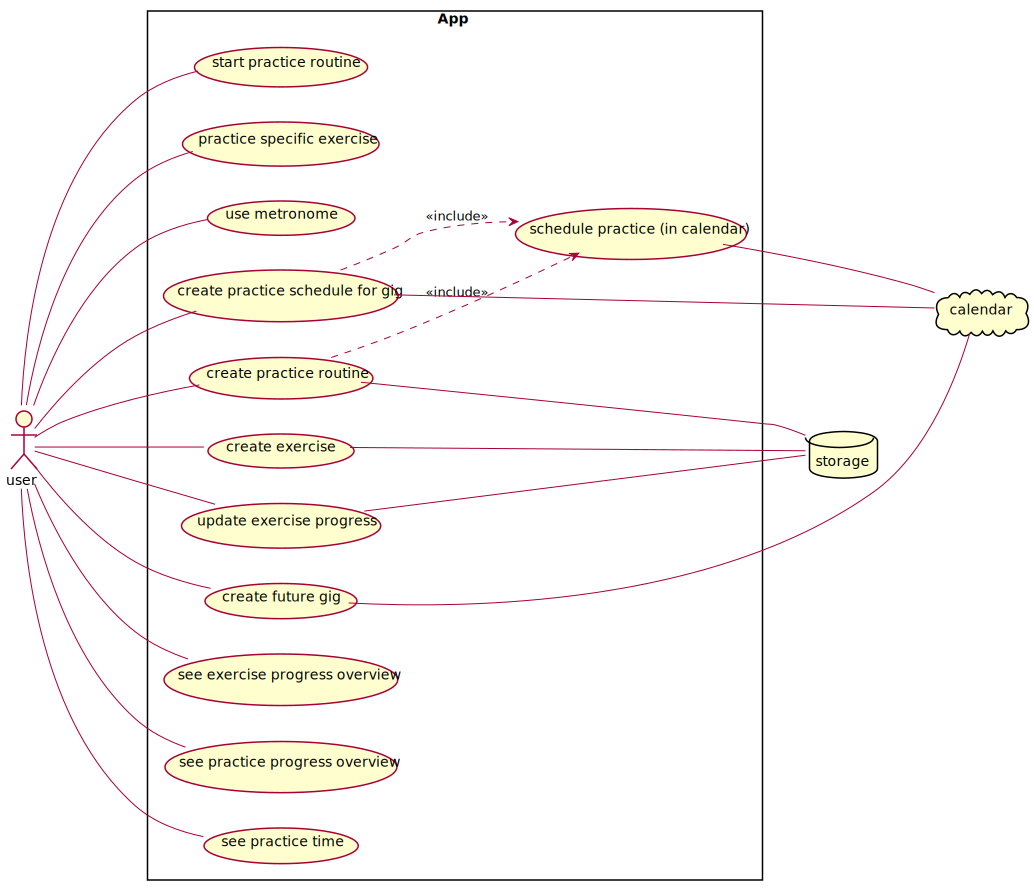
\includegraphics[width=12cm]{usecases1.png}
\caption{Usecase diagram}
\end{figure}

\begin{table}[htp]
\caption{Use Case (ID: U-01): Usecase Name}\label{U-01}
\begin{tabular}{lp{10cm}}
  \hline
  \textbf{Title:}             & Usecase Name \\
  \hline
  \textbf{Primary Actor:}     & Bikefitter \/ user \\
  \hline
  \textbf{Success Scenario:}  & 1.~Benutzer wählt Datenverzeichnis \\
                              & 2.~Benutzer wählt durzuführende Analysen \\
                              & 3.~Benutzer wählt Ergebnisverzeichnis \\
                              & 4.~System berechnet Werte \\
  \hline
  \textbf{Requirement:}       & Anwendung gestartet \\
  \hline
\end{tabular}
\end{table}

\begin{appendix}
  \listoftables
\end{appendix}
\end{document}
